% \vspace{-0.5em}
%-------------------------------------
\section{Agentic Data Harmonization}
\label{sec:agentic-data-harmonization}
%-------------------------------------

% \begin{figure}[ht]
%      \centering
%      \begin{subfigure}{0.9\linewidth}
%      \centering
%             \begin{tikzpicture}
%             \tikzstyle{vertex}=[circle,fill=none,draw=black,minimum size=17pt,inner sep=0pt]
% \node[vertex] (S) at (0,0) {$S$};
% \node[vertex] (A) at (2,0) {$A$};
% \node[vertex] (D) at (1,1) {$D$};
% \path (S) edge (D);
% \path (D) edge (A);
% \path[red] (S) edge (A);
%             \end{tikzpicture}
%         \caption{Causal graph for $\model \in \modelsunconfedge$ illustrating all possible functional dependencies.}
%         \label{fig:no-cf-edge}
%         \end{subfigure}    \hfill
% %              \begin{subfigure}{0.45\linewidth}
% %              \centering
% %             \begin{tikzpicture}
% %             \tikzstyle{vertex}=[circle,fill=none,draw=black,minimum size=17pt,inner sep=0pt]
% % \node[vertex] (S) at (0,0) {$S$};
% % \node[vertex] (A) at (2,0) {$A$};
% % \node[vertex] (D) at (1,1) {$D$};
% % \path (S) edge (D);
% % \path (D) edge (A);
% % %\path[red] (S) edge (A);
% %             \end{tikzpicture}
% %         \caption{Causal graph for $\model \in \nullgraphunconf$ illustrating all possible functional dependencies.}
% %         \label{fig:no-cf-no-edge}
% %         \end{subfigure}
% \end{figure}

% \begin{figure}[h]
%      \centering
%             \begin{tikzpicture}
%             \tikzstyle{vertex}=[circle,fill=none,draw=black,minimum size=17pt,inner sep=0pt]
% \node[vertex] (S) at (0,0) {$S$};
% \node[vertex] (A) at (2,0) {$A$};
% \node[vertex] (D) at (1,1) {$D$};
% \path (S) edge (D);
% \path (D) edge (A);
% \path[bidirected] (D) edge[bend left=60] (A);
% \path[red] (S) edge (A);
% % \draw[->, line width=0.3mm]  (S)--(D);
% % \draw[->, line width=0.3mm]  (D)--(A);
% % \draw[->, line width=0.3mm]  (S)--(A);
% % \draw[<->, line width=0.3mm]  (D)--(A);
%             \end{tikzpicture}
%         \caption{Causal graph for $\model \in \modelsunconfedge$ illustrating all possible functional dependencies.}
%         \label{fig:cf-no-edge}
% \end{figure}

% \begin{figure}[h]
%      \centering
%             \begin{tikzpicture}
%             \tikzstyle{vertex}=[circle,fill=none,draw=black,minimum size=17pt,inner sep=0pt]
% \node[vertex] (S) at (0,0) {$S$};
% \node[vertex] (A) at (3,-0.5) {$A$};
% \node[vertex] (D) at (1,1) {$D$};
% \node[vertex] (S') at (1,-0.5) {$S'$};
% \path (S) edge (D);
% \path (D) edge (A);
% \path[bidirected] (D) edge[bend left=60] (A);
% \path[red] (S') edge (A);
% %\path (S) edge (S'); 
%  \path (S) edge node[near start, below] {=} (S');
% % \draw[->, line width=0.3mm]  (S)--(D);
% % \draw[->, line width=0.3mm]  (D)--(A);
% % \draw[->, line width=0.3mm]  (S)--(A);
% % \draw[<->, line width=0.3mm]  (D)--(A);
%             \end{tikzpicture}
%         \caption{Causal graph for $\model \in \modelsedge$ illustrating all possible functional dependencies.} 
%         \label{fig:cf-edge}
% \end{figure}


%              \begin{subfigure}{0.45\linewidth}
%              \centering
%             \begin{tikzpicture}
%             \tikzstyle{vertex}=[circle,fill=none,draw=black,minimum size=17pt,inner sep=0pt]
% \node[vertex] (S) at (0,0) {$S$};
% \node[vertex] (A) at (2,0) {$A$};
% \node[vertex] (D) at (1,1) {$D$};
% \path (S) edge (D);
% \path (D) edge (A);
% %\path[red] (S) edge (A);
%             \end{tikzpicture}
%         \caption{Causal graph for $\model \in \nullgraphunconf$ illustrating all possible functional dependencies.}
%         \label{fig:no-cf-no-edge}
%         \end{subfigure}
%\end{figure}

\begin{figure*}[t]
     \centering
     \begin{subfigure}{0.32\linewidth}
     \centering
            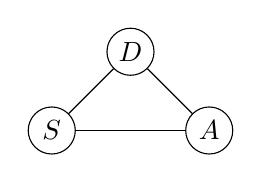
\begin{tikzpicture}
            \tikzstyle{vertex}=[circle,fill=none,draw=black,minimum size=17pt,inner sep=0pt]
\node[vertex] (S) at (0,0) {$S$};
\node[vertex] (A) at (2,0) {$A$};
\node[vertex] (D) at (1,1) {$D$};
\path (S) edge (D);
\path (D) edge (A);
\path (S) edge (A);
            \end{tikzpicture}
        \caption{$\model \in \modelsunconfedge$}
        \label{fig:no-cf-edge}
\end{subfigure}
     \begin{subfigure}{0.32\linewidth}
     \centering
            \begin{tikzpicture}
            \tikzstyle{vertex}=[circle,fill=none,draw=black,minimum size=17pt,inner sep=0pt]
\node[vertex] (S) at (0,0) {$S$};
\node[vertex] (A) at (2,0) {$A$};
\node[vertex] (D) at (1,1) {$D$};
%\node[vertex] (S') at (1,-0.5) {$S'$};
\path (S) edge (D);
\path (D) edge (A);
\path[bidirected] (D) edge[bend left=60] (A);
\path (S) edge (A);
%\path (S) edge (S'); 
% \path (S) edge node[near start, below] {=} (S');
% \draw[->, line width=0.3mm]  (S)--(D);
% \draw[->, line width=0.3mm]  (D)--(A);
% \draw[->, line width=0.3mm]  (S)--(A);
% \draw[<->, line width=0.3mm]  (D)--(A);
            \end{tikzpicture}
        \caption{$\model \in \modelsedgerelax$} 
        \label{fig:cf-edge}
        \end{subfigure}
         \begin{subfigure}{0.32\linewidth}
     \centering
            \begin{tikzpicture}
            \tikzstyle{vertex}=[circle,fill=none,draw=black,minimum size=17pt,inner sep=0pt]
\node[vertex] (S) at (0,0) {$S$};
\node[vertex] (A) at (2,0) {$A$};
\node[vertex] (D) at (1,1) {$D$};
%\node[vertex] (S') at (1,-0.5) {$S'$};
\path (S) edge (D);
\path (D) edge (A);
\path[bidirected] (D) edge[bend left=60] (A);
%\path (S) edge (A);
%\path (S) edge (S'); 
% \path (S) edge node[near start, below] {=} (S');
% \draw[->, line width=0.3mm]  (S)--(D);
% \draw[->, line width=0.3mm]  (D)--(A);
% \draw[->, line width=0.3mm]  (S)--(A);
% \draw[<->, line width=0.3mm]  (D)--(A);
            \end{tikzpicture}
        \caption{$\model \in \nullgraph$ and $\model \in \modeliv$} 
        \label{fig:cf-edge-iv}
        \end{subfigure}
        \caption{Causal graphs, $\cg{\model}$, assumed in various model classes.}
\end{figure*}

% \begin{figure}
%      \centering
%             \begin{tikzpicture}
%             \tikzstyle{vertex}=[circle,fill=none,draw=black,minimum size=17pt,inner sep=0pt]
% \node[vertex] (Z) at (0,0) {$Z$};
% \node[vertex] (Y) at (3,0) {$Y$};
% \node[vertex] (X) at (1.5,0) {$X$};
% %\node[vertex] (S') at (1,-0.5) {$S'$};
% \path (Z) edge (X);
% \path (X) edge (Y);
% \path[bidirected] (X) edge[bend left=60] (Y);
% %\path[red] (S') edge (A);
% %\path (S) edge (S'); 
%  %\path (S) edge node[near start, below] {=} (S');
% % \draw[->, line width=0.3mm]  (S)--(D);
% % \draw[->, line width=0.3mm]  (D)--(A);
% % \draw[->, line width=0.3mm]  (S)--(A);
% % \draw[<->, line width=0.3mm]  (D)--(A);
%             \end{tikzpicture}
%         \caption{Causal graph of $M \in \modeliv$} 
%         \label{fig:iv}
%         \end{figure}

% LLM-based agents integrate the capabilities of language models with reasoning, planning, memory retention, and interaction with external tools~\cite{qin2024toolllm,code-generatingLLMCHI23}.
We propose using LLM-based agents to facilitate the interactive construction of harmonization pipelines through natural language and visual interfaces. We aim to simplify the harmonization process and empower domain experts to harmonize their own data~effectively.

Our approach has three main aspects -- \textit{harmonization primitives}, \textit{harmonization agents}, and \textit{human-agent interaction}, as illustrated in Figure~\ref{fig:system-diagram}. 
The system should support two-way interaction between the \textit{users} and the \textit{harmonization agents}. While the former drives the system and defines the tasks to be performed, the latter aims to automate most data harmonization tasks, leaving only key decisions that need external context to users.
By capturing user-agent interactions and the derived computational pipelines, we maintain the provenance of the harmonization process. This supports transparency and reproducibility, making it possible to publish the harmonized data with the pipeline used to derive it.

\myparagraph{Harmonization Primitives}
The bottom of Figure~\ref{fig:system-diagram} illustrates a library of components that we refer to as \textit{data integration primitives}. These are key algorithms or routines that can be developed to solve well-defined data integration tasks such as schema matching, value matching, % function-attribute matching,
and others. Some of these components are lower-level routines that support other higher-level tasks, e.g., column-type annotation may be a component of schema-matching algorithms~\cite{feuer:vldb2024}, and entity resolution and deduplication may be key to performing data standardization~\cite{christophides2020overview}. While the particular set of primitives can be heterogeneous and evolve to support the system capabilities, they have in common that they need to be \textit{composable} and can be invoked by both user and AI agents.

\textit{Primitive composability} refers to the ability to combine primitives to create a pipeline: the output of a primitive $p_1$ can be used as input of another primitive $p_2$. For example, \textit{schema matching} primitives can output a list of source-target attribute pairs.
These lists form the input for the \textit{value matching} primitives, which then find equivalences between the values of the source attribute to the target. Finally, the output of value-matching primitives can be used to assemble a \textit{harmonization specification} that describes the transformation of source tables $T_i$ into a target output table $T_{target}$.
% 
In short, primitive composability enables the creation of data harmonization pipelines by allowing the chaining of operations that take source tables as input and produce harmonized data as output.

\myparagraph{Data Harmonization Agents}
The harmonization agent fulfills user requests by synthesizing pipelines that perform the requested harmonization task. 
First, it decomposes the problem in a sequence of actions. These actions can be of multiple types, including execution of existing integration primitives (tool calling) or execution of code generated on-demand. 
To decide on what action to take, the harmonization agent leverages an LLM, which is provided with descriptions of the task and integration primitives available for use. 
The LLM then returns an action (e.g., a code snippet) that can be executed in a runtime environment (e.g., a Python kernel). The action output is then fed back into the LLM, which decides if it needs to execute additional actions or if the task is completed.
This loop executes until the task is deemed complete (see Figure~\ref{fig:agent-loop}).
% As illustrated in Figure~\ref{fig:agent-loop}, this loop executes until the task is deemed complete 

The main loop is orchestrated by a driver code that takes inputs from the user (i.e., prompts) that describe the task to be performed. 
This driver is also responsible for (1) communicating with users to request inputs (e.g., when the LLM asks for task clarification or user preferences) and (2) managing the state (memory) of the agent. For example, it can also track and store the history of actions and user interactions in a \textit{Provenance DB}.
This data can support decisions about future actions, and transparency, and be used to generate harmonization \textit{specifications} or scripts to reproduce the results.

Given the complexity of harmonization tasks, it is crucial to have high-level primitives available as building blocks for the pipeline.
This allows encoding prior knowledge and using efficient algorithms known to be effective for a specific task.
These primitives encompass algorithms for tasks such as schema matching, entity resolution, and value mapping. Of course, primitives can go beyond hard-coded functions that implement deterministic algorithms. For instance, they can be workflows that use LLMs to perform specific tasks such as in \cite{liu2024magneto} or they could generate code on demand (e.g., to extract data from or to transform attribute values~\cite{autoformula2024}). 


\myparagraph{Human-Agent Interaction}
A central component of our system architecture is the user-agent interaction. We argue that systems must go beyond text-based conversational interactions: they need to support rich visual data representations and should allow interactions that help users reason about the answers produced by the agent and refine the task definition as well as the pipelines derived by the agent. In complex tasks such as harmonization, this is necessary since many decisions needed to complete the task (e.g., whether two terms represent the same concept) are difficult even for domain experts and may require external knowledge, such as the context in which data was collected.

In this paper, we focus on interactions based on natural language via a chatbot interface. However, it should be possible to implement even more intuitive and efficient graphical interfaces that combine natural language with point-and-click components. For example, as done in interactive AutoML tools~\cite{santos2019visus}, the system may guide the user through the harmonization process, recommend the available actions, track progress, and provide data visualizations to help the user better make sense of the data. This may help prevent common issues in natural language such as ambiguity~\cite{esfandiarpoor2024followup}.

\vspace{-.75em}
\section{System Prototype \& Use Case} \label{sec:prototype}

\myparagraph{The primitives library}
% We used the data harmonization primitives provided by \texttt{bdi-kit} \cite{bdi-kit-github}, an open-source Python library. 
We used data harmonization primitives from \texttt{bdi-kit} \cite{bdi-kit-github}, an open-source Python library that we designed with the explicit goal of composability.
%We implemented the data harmonization primitives library in Python and released it as the Python library that we call \texttt{bdi-kit} \cite{bdi-kit-github}. 
Currently, it includes implementations of multiple \textit{schema matching} and \textit{value matching} algorithms using a composable API. It includes several classic algorithms from Koutras et al.~\cite{koutras2021valentine} and language model-based algorithms such as the ones presented in~\cite{liu2024enhancing} and \cite{liu2024magneto}. Most functions take as input a \texttt{source} parameter that represents the user's input DataFrame and returns the output formatted as another DataFrame. The \texttt{target} parameter can either be a string representing a target standard schema (e.g., \texttt{`gdc'}) or a target DataFrame, this allows switching between the two tasks described in Examples~\ref{example1} and ~\ref{example2}. Figure~\ref{fig:bdi-kit} shows a subset of functions relevant to this paper.

\begin{figure}[t]
% \vspace{-1.25em}
\centering
\begin{tcolorbox}[colback=black!2.5!white,colframe=black!85!black,boxrule=0.25mm,boxsep=4pt,left=0pt,right=0pt,top=0pt,bottom=0pt]

    \footnotesize
    
    \texttt{\textbf{match\_schema}(source, target, method, ...)} \\
    Maps the schema of a source table to a target schema (table or predefined standard like \texttt{gdc}) using a specified method.
    \vspace{.5em}
    
    
    \texttt{\textbf{top\_matches}(source, column, target, top\_k, method, ...)} \\
    Finds the top-\texttt{k} matches between a source column and columns of a target schema.
    \vspace{.5em}
    
    
    \texttt{\textbf{match\_values}(source, target, column\_mapping, method, ...)} \\
    Matches values between columns of a source and a target using a specified method, returning one or more result tables.
    \vspace{.5em}
    
    
    % \texttt{\textbf{top\_value\_matches}(source, target, column\_mapping, top\_k,...)} \\ %  method, 
    % Finds the top-\texttt{k} value matches between columns in a source and target.
    % \vspace{.5em}
    
    
    % \texttt{\textbf{view\_value\_matches}(matches, edit = False)} \\
    % Displays value match results in a table format, with optional editing.
    % \vspace{.5em}

    
    % \texttt{\textbf{preview\_domain}(dataset, column, limit = None) → DataFrame} \\
    % Previews unique values and descriptions in a specified column of a dataset.
    % \vspace{.5em}

    
    % \texttt{\textbf{merge\_mappings}(mappings, user\_mappings = None) → List} \\
    % Combines computed and user-provided mappings into a plan for data transformation.
    % \vspace{.5em}

    
    \texttt{\textbf{materialize\_mapping}(input\_table, mapping\_spec) → DataFrame} \\
    Transforms a source table into a new table using a mapping specification.
    % 
    % \texttt{create\_mapper(input) → ValueMapper} \\
    % Creates a mapper object for transforming column values based on the input type. \\
    
    % \texttt{MappingSpecLike} \\
    % Defines mappings between source and target columns, including optional value transformations. \\
\end{tcolorbox}
% \vspace{-1.5em}
\caption{A subset of functions available in the \texttt{bdi-kit} API.}
% \vspace{-1.5em}
\label{fig:bdi-kit}
\end{figure}

\myparagraph{The data harmonization agent} We implemented \systemname, a system prototype that uses the data integration primitives from Figure~\ref{fig:bdi-kit} and interacts with users via a text-based chat box. Implementing an agent entails writing carefully crafted function and task descriptions that are combined to assemble system prompts fed to the LLMs. For our prototype, we implemented tool wrappers for each of the \texttt{bdi-kit} functions, along with descriptions of when each should be used. We also provide general descriptions of the data harmonization steps, when the LLM should request help from the user, and output formatting instructions.

To implement the tool calling functionality and the user interface, we used the Archytas~\cite{archytas} library, an open-source tool for building AI agents based on the ReAct framework~\cite{yao2022react}, and Beaker~\cite{beaker}, a contextually-aware notebook system that supports the development of chatbot user interfaces. This allows us to implement features that facilitate interaction, such as rendering markdown-formatted outputs in the browser, displaying the reasoning steps taken by the agent, collecting user inputs, and feeding them back to the agent.

%\myparagraph{Use case: harmonization with the GDC standard} % previous title
\myparagraph{Human-agent interaction: The GDC use case}
To demonstrate the ability to produce good data harmonization plans, we present a use case that harmonizes a dataset from Dou et al.~\cite{dou2020proteogenomic} (described in Example~\ref{example1}) with the GDC standard. 
% Below we provide an example of interaction with the chatbot agent.
Below, we show message exchanges between the user ({\scriptsize \faUser}) and the agent ({\scriptsize \faRobot}), along with explanations of the actions taken by the agent to answer user queries.

The user starts by requesting the system to load a CSV file that contains the attributes of interest:
% \vbox{
% \vspace{-.5em}
\chatboxUser{
Load the file dou.csv as a dataframe and subset it to the following columns: Country, Histologic\_Grade\_FIGO, Histologic\_type, FIGO\_stage, BMI, Age, Race, Ethnicity, Gender, Tumor\_Focality, Tumor\_Size\_cm.
}
% \vspace{-1em}
\chatboxAgent{
The file 'dou.csv' has been successfully loaded and subsetted to the specified columns: Country, Histologic\_Grade\_FIGO, Histologic\_type, FIGO\_stage, BMI, Age, Race, Ethnicity, Gender, Tumor\_Focality, Tumor\_Size\_cm.\\
Outputs:\\
{\color{gray}[...data frame displayed here...]}
}
\vspace{-.5em}
% }
\noindent Responding to this prompt, the agent automatically (1) generates Python code using the Pandas library that loads and selects the requested columns and (2) executes the generated code to load the CSV file into memory. This example illustrates the capability of \textit{on-demand code generation} to accomplish a requested task.

Next, the user requests the system to perform schema matching between the table loaded and the attributes from the GDC standard:

% \vspace{-.5em}
\chatboxUser{
Please match this to the GDC schema using the `ct\_learning' method, and fix any results that don't look correct.
}
% \vspace{-.5em}

\noindent
As shown in Figure~\ref{fig:sequence-diagram}, the system interacts with an LLM multiple times to answer this request. First, it sends the initial user's prompt to the LLM, which recognizes that the function \texttt{match\_schema} is adequate to solve the request, and thus returns a tool calling instruction containing the \texttt{match\_schema} function name along with the needed parameters. Note that the LLM parses the user's query, and recognizes that \texttt{gdc} must be used as the target schema and \texttt{ct\_learning} refers to the argument \texttt{method} of \texttt{match\_schema()}. 
% 
After receiving the tool calling instruction as output, the system then executes the primitive function requested by the LLM, collects the list of column matches returned, and passes it back to the LLM in a follow-up prompt. 

After analyzing the column match results received in the follow-up prompt, the LLM detects a mapping mistake for the column \texttt{Histologic\_type}, which is wrongly mapped to \texttt{roots}. To fix the error, the LLM triggers a tool calling instruction that uses the primitive function \texttt{top\_matches} to find the top~10 alternative candidates for \texttt{Histologic\_type}. After receiving the results, it analyzes the results and suggests using \texttt{primary\_diagnosis} as a correction to the user (who agrees) as seen in the following messages:

\vbox{
% \vspace{-.5em}
\chatboxAgent{The current mapping for `Histologic\_type' is `roots', which seems incorrect. The top alternatives are:\\
- history\_of\_tumor\_type\\
- primary\_diagnosis\\
- sample\_type\\
I suggest using `primary\_diagnosis'. Do you agree with this choice?
}
% \vspace{-1em}
\chatboxUser{yes}
}
\vspace{-.5em}
\noindent 
As a final response to the task, the agent shows a table of column mappings as output, where the ``\texttt{Source Column}'' contains columns from the source table (\texttt{dou.csv}), ``\texttt{Target Column}'' contains a column match from the GDC standard, and ``\texttt{Corrected?}'' indicates whether the LLM has corrected the original \texttt{bdi-kit} match.

\vspace{-.25em}
\chatboxAgent{
Result:\\

% \scriptsize
\vspace{-0.25em}
\hspace{-0.25cm}
\begin{tabular}{lll}
\textbf{Source Column} & \textbf{Target Column} & \textbf{Corrected?} \\
Country & country\_of\_birth & No \\
Histologic\_Grade\_FIGO & tumor\_grade & No \\
Histologic\_type & primary\_diagnosis & Yes, from ``roots'' \\
FIGO\_stage & figo\_stage & No \\
BMI & bmi & No \\
Age & age\_at\_onset & No \\
Race & race & No \\
Ethnicity & ethnicity & No \\
Gender & gender & No \\
Tumor\_Focality & tumor\_focality & No \\
Tumor\_Size\_cm & tumor\_depth\_measurement & No \\
\end{tabular}
}
% }

Since the user is a domain expert who knows the GDC standard and knows that there may be better options for \texttt{Tumor\_Size\_cm}, it asks the system to find an alternative match. The system then updates the previous list with a more appropriate match found using the \texttt{top\_matches} function. This interaction is shown next:

\vbox{
% \vspace{-.25em}
\chatboxUser{
Find alternative mappings for Tumor\_Size\_cm.
}
% \vspace{-1em}
\chatboxAgent{Result:\\

\scriptsize
\vspace{-0.25em}
\hspace{-0.25cm}
\begin{tabular}{lll}
    \textbf{Source Column} & \textbf{Target Column} & \textbf{Corrected?} \\ 
    {\color{gray}[...]} & {\color{gray}[...]} & {\color{gray}[...]} \\
    % Country & country\_of\_birth & No \\ 
    % Histologic\_Grade\_FIGO & tumor\_grade & No \\ 
    % Histologic\_type & primary\_diagnosis & Yes, from "roots" \\ 
    % FIGO\_stage & figo\_stage & No \\ 
    % BMI & bmi & No \\ 
    % Age & age\_at\_onset & No \\ 
    % Race & race & No \\ 
    % Ethnicity & ethnicity & No \\ 
    % Gender & gender & No \\ 
    Tumor\_Focality & tumor\_focality & No \\ 
    % Tumor\_Size\_cm & tumor\_largest\_dimension\_diameter & Yes, from "tumor\_depth\_measurement" \\ 
    Tumor\_Size\_cm & tumor\_largest\_dimension\_diameter & Yes, from "tumor\_depth... \\ 
\end{tabular}
}
} %\vbox

% --------------
% Value mappings
% --------------

After finding correct matches for all source columns, the next step is to find value mappings for each column match. The following prompt requests the agent to find such mappings:

% \vspace{-0.75em}
% \vbox{
\chatboxUser{\raggedright Find value mappings for the columns Country, Histologic\_Grade\_FIGO, Histologic\_type, FIGO\_stage, Race, Ethnicity, Gender, Tumor\_Focality. If there are any errors in the mappings, please provide suggestions.
}
% \vspace{-0.75em}
\noindent
As in the previous prompts, finding value mappings requires multiple LLM interactions. First, the LLM triggers one function call of \texttt{match\_values()} for each of the source-target column pairs using the default value matching method \texttt{tfidf}  (an efficient algorithm that chooses matches based on the tf-idf similarity over character n-grams). After receiving the value matches, the LLM evaluates if they are correct, and fixes the entries that contain errors. To do so, it calls another function to discover the list of acceptable values in a GDC attribute and picks the correct one. A snippet of the result is shown next (we omit part of the output due to lack of space):
%in the box below:

\vspace{-0.5em}
\chatboxAgent{\scriptsize
{\color{gray}[...]}\\

\vspace{-0.5em}
\textbf{Histologic\_Grade\_FIGO → tumor\_grade}\\

\vspace{-0.5em}
\hspace{-0.25cm}
\begin{tabular}{lll}
    \textbf{Source Value} & \textbf{Target Value} & \textbf{Corrected?} \\ 
    FIGO grade 1 & G1 & Yes, from "Low Grade" \\ 
    FIGO grade 2 & G2 & Yes, from "Low Grade" \\ 
    FIGO grade 3 & G3 & Yes, from "Low Grade" \\ 
\end{tabular}\\

{\color{gray}[...]}\\

\vspace{-0.25em}
\textbf{FIGO\_stage → figo\_stage}\\

\vspace{-0.25em}
\hspace{-0.25cm}
\begin{tabular}{lll}
    \textbf{Source Value} & \textbf{Target Value} & \textbf{Corrected?} \\ 
    IIIC2 & Stage IIIC2 & No \\ 
    IIIC1 & Stage IIIC1 & No \\ 
    IVB & Stage IVB & No \\ 
    IIIB & Stage IIIB & No \\ 
    IIIA & Stage IIIA & No \\ 
    II & Stage II & Yes, from "Stage III" \\ 
\end{tabular}\\

\vspace{-0.25em}
{\color{gray}[...]}
}
% \vspace{-0.5em}
% }

\noindent
This example illustrates the ability of the LLM to detect and correct errors automatically without the user's intervention. As an example, it corrects the match $\langle\texttt{II}, \texttt{Stage III}\rangle$ to $\langle\texttt{II}, \texttt{Stage II}\rangle$. This showcases how we can leverage existing fast algorithms to perform most of the work while leveraging LLMs as an evaluator that can detect and fix mistakes only when needed.

% ------------------
% Materialize schema
% ------------------

The final step is generating a harmonized table. The boxes below show the user prompt as well as the agent response:

\vbox{
% \vspace{-0.25em}
\chatboxUser{Please create a final harmonized table based on the discovered column and value mappings and save it at "dou\_harmonized.csv".}
% \vspace{-1em}
\chatboxAgent{The harmonized table has been successfully created and saved as `dou\_harmonized.csv'.}
% \vspace{-0.25em}
}
\noindent
In this example, the agent uses \texttt{materialize\_mapping} to generate a table and save file \texttt{`dou\_harmonized.csv'}. The LLM  first creates a declarative mapping specification according to the bdi-kit's format used to describe a harmonization plan. Figure~\ref{fig:mapping-spec} shows a snippet of the generated harmonization plan, which includes a declarative specification of the mappings to be performed written in JSON. In this example, we only show dictionary-based transformations that map source values into target values. However, bdi-kit's also supports other types of transformations, such as custom mappings that take as input a custom Python function (or lambda).
This can potentially be used along with the on-demand code generation.

The main advantage of using a declarative language to describe harmonization plans is that it enables reproducibility: once a plan is created, users can feed the plan along with the source data into \texttt{materialize\_mapping} function to recreate the harmonized data. This does not require re-running any LLM-based interactions, since all transformations are encoded in the harmonization plan.

% This is a hack to remove the syntax highlighting error in the minted box below
\AtBeginEnvironment{minted}{\renewcommand{\fcolorbox}[4][]{#4}}
\begin{figure}[h]
\vspace{-.75em}
\begin{tcolorbox}[colback=black!2.5!white,colframe=black!85!black,boxrule=0.25mm,boxsep=4pt,left=0pt,right=0pt,top=0pt,bottom=0pt]
\begin{minted}[fontsize=\scriptsize]{json}
[ 
 [...]
 { "source": "Country",
   "target": "country_of_birth",
   "matches": [ ["United States", "United States"],
                ["Poland", "Poland"],
                ["Ukraine", "Ukraine"] ] },
 { "source": "Histologic_Grade_FIGO",
   "target": "tumor_grade",
   "matches": [ ["FIGO grade 1", "G1"],
                ["FIGO grade 2", "G2"],
                ["FIGO grade 3", "G3"] ] },
 [...]
]
\end{minted}
\end{tcolorbox}
\vspace{-1.25em}
\caption{A snippet from the mapping specification generated that is passed to \texttt{materialize\_mapping()} function.}
\label{fig:mapping-spec}
\end{figure}